% === Bayesian Posterior Table ===
\begin{table}[t]
\centering
\caption{Bayesian posterior analysis: Beta-Binomial model with uniform prior. $k$=passes, $n$=trials, posterior Beta$(1{+}k, 1{+}n{-}k)$.}
\label{tab:bayesian-posteriors}
\begin{tabular}{llrrrrr}
\toprule
Model & Mode & $k/n$ & Post.\ mean & 95\% HDI low & 95\% HDI high \\
\midrule
  M2.1 & d0-i1 & 0/8 & 0.100 & 0.003 & 0.341 \\
  M2.1 & d1-i3 & 3/8 & 0.400 & 0.137 & 0.701 \\
  M2.1 & d6-i1 & 0/8 & 0.100 & 0.003 & 0.341 \\
  M2.1 & d0-i3 & 3/8 & 0.400 & 0.137 & 0.701 \\
  M2.5 & d0-i1 & 0/8 & 0.100 & 0.003 & 0.341 \\
  M2.5 & d1-i3 & 3/8 & 0.400 & 0.137 & 0.701 \\
  M2.5 & d6-i1 & 0/8 & 0.100 & 0.003 & 0.341 \\
  M2.5 & d0-i3 & 4/8 & 0.500 & 0.212 & 0.788 \\
  Qwen3-235B & d0-i1 & 0/8 & 0.100 & 0.003 & 0.341 \\
  Qwen3-235B & d1-i3 & 3/8 & 0.400 & 0.137 & 0.701 \\
  Qwen3-235B & d6-i1 & 0/8 & 0.100 & 0.003 & 0.341 \\
  Qwen3-235B & d0-i3 & 2/8 & 0.300 & 0.075 & 0.600 \\
  Qwen3.5 & d0-i1 & 0/8 & 0.100 & 0.003 & 0.341 \\
  Qwen3.5 & d1-i3 & 6/8 & 0.700 & 0.400 & 0.925 \\
  Qwen3.5 & d6-i1 & 0/8 & 0.100 & 0.003 & 0.341 \\
  Qwen3.5 & d0-i3 & 1/8 & 0.200 & 0.028 & 0.483 \\
  DSV3.2 & d0-i1 & 0/8 & 0.100 & 0.003 & 0.341 \\
  DSV3.2 & d1-i3 & 4/8 & 0.500 & 0.212 & 0.788 \\
  DSV3.2 & d6-i1 & 0/8 & 0.100 & 0.003 & 0.341 \\
  DSV3.2 & d0-i3 & 3/8 & 0.400 & 0.137 & 0.701 \\
  Kimi-K2 & d0-i1 & 0/8 & 0.100 & 0.003 & 0.341 \\
  Kimi-K2 & d1-i3 & 3/8 & 0.400 & 0.137 & 0.701 \\
  Kimi-K2 & d6-i1 & 0/8 & 0.100 & 0.003 & 0.341 \\
  Kimi-K2 & d0-i3 & 2/8 & 0.300 & 0.075 & 0.600 \\
  K2.5 & d0-i1 & 5/8 & 0.600 & 0.299 & 0.863 \\
  K2.5 & d1-i3 & 4/8 & 0.500 & 0.212 & 0.788 \\
  K2.5 & d6-i1 & 5/8 & 0.600 & 0.299 & 0.863 \\
  K2.5 & d0-i3 & 6/8 & 0.700 & 0.400 & 0.925 \\
\bottomrule
\end{tabular}
\end{table}

% === Bayesian HDI Figure ===
\begin{figure}[t]
\centering
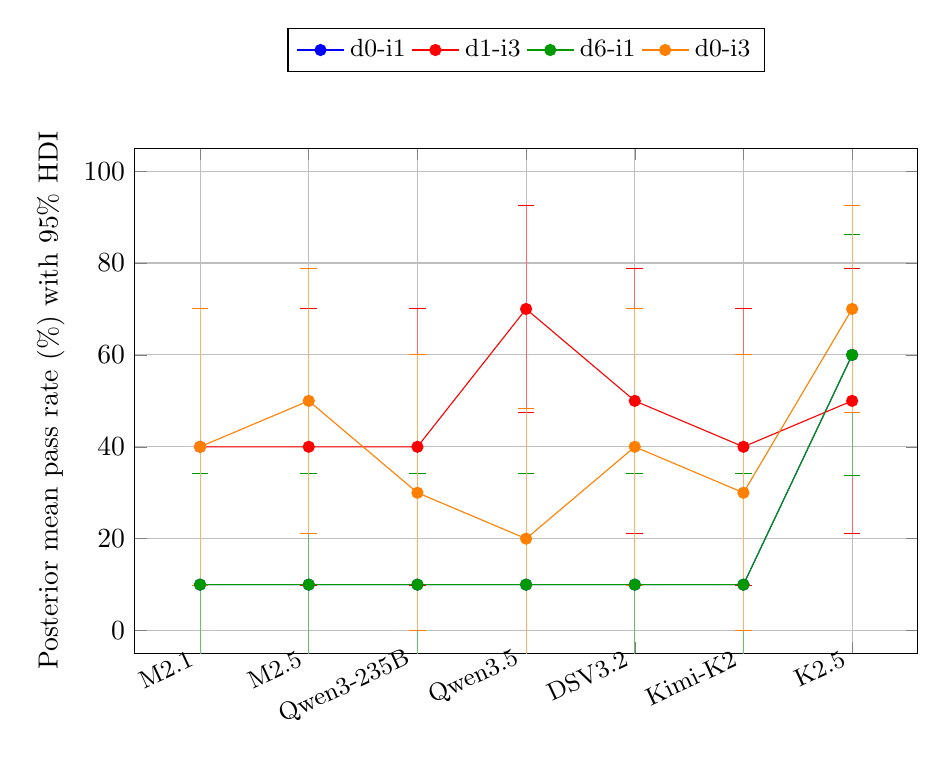
\begin{tikzpicture}
\begin{axis}[
  width=0.95\linewidth,
  height=8cm,
  ymin=-5, ymax=105,
  ylabel={Posterior mean pass rate (\%) with 95\% HDI},
  symbolic x coords={M2.1,M2.5,Qwen3-235B,Qwen3.5,DSV3.2,Kimi-K2,K2.5},
  xtick=data,
  x tick label style={rotate=25,anchor=east,font=\small},
  legend style={at={(0.5,1.15)},anchor=south,legend columns=4,font=\small},
  grid=major,
]
\addplot[blue,mark=*,mark size=2pt,error bars/.cd,y dir=both,y explicit,
  error bar style={blue!60},error mark options={rotate=90,mark size=3pt,blue}]
  coordinates {
      (M2.1,10.0) +- (0,24.1)
      (M2.5,10.0) +- (0,24.1)
      (Qwen3-235B,10.0) +- (0,24.1)
      (Qwen3.5,10.0) +- (0,24.1)
      (DSV3.2,10.0) +- (0,24.1)
      (Kimi-K2,10.0) +- (0,24.1)
      (K2.5,60.0) +- (0,26.3)
  };
\addplot[red,mark=*,mark size=2pt,error bars/.cd,y dir=both,y explicit,
  error bar style={red!60},error mark options={rotate=90,mark size=3pt,red}]
  coordinates {
      (M2.1,40.0) +- (0,30.1)
      (M2.5,40.0) +- (0,30.1)
      (Qwen3-235B,40.0) +- (0,30.1)
      (Qwen3.5,70.0) +- (0,22.5)
      (DSV3.2,50.0) +- (0,28.8)
      (Kimi-K2,40.0) +- (0,30.1)
      (K2.5,50.0) +- (0,28.8)
  };
\addplot[green!60!black,mark=*,mark size=2pt,error bars/.cd,y dir=both,y explicit,
  error bar style={green!60!black!60},error mark options={rotate=90,mark size=3pt,green!60!black}]
  coordinates {
      (M2.1,10.0) +- (0,24.1)
      (M2.5,10.0) +- (0,24.1)
      (Qwen3-235B,10.0) +- (0,24.1)
      (Qwen3.5,10.0) +- (0,24.1)
      (DSV3.2,10.0) +- (0,24.1)
      (Kimi-K2,10.0) +- (0,24.1)
      (K2.5,60.0) +- (0,26.3)
  };
\addplot[orange,mark=*,mark size=2pt,error bars/.cd,y dir=both,y explicit,
  error bar style={orange!60},error mark options={rotate=90,mark size=3pt,orange}]
  coordinates {
      (M2.1,40.0) +- (0,30.1)
      (M2.5,50.0) +- (0,28.8)
      (Qwen3-235B,30.0) +- (0,30.0)
      (Qwen3.5,20.0) +- (0,28.3)
      (DSV3.2,40.0) +- (0,30.1)
      (Kimi-K2,30.0) +- (0,30.0)
      (K2.5,70.0) +- (0,22.5)
  };
\legend{d0-i1,d1-i3,d6-i1,d0-i3}
\end{axis}
\end{tikzpicture}
\caption{Bayesian 95\% highest-density intervals for pass rate by model and mode. Points show posterior mean; bars show 95\% credible interval under Beta(1,1) prior. Wide intervals reflect $n{=}8$ trials per configuration.}
\label{fig:bayesian-hdi}
\end{figure}

% === Thompson Sampling Table ===
\begin{table}[t]
\centering
\caption{Thompson sampling selection probability per model (10{,}000 rounds). Higher values indicate the mode is more likely to be optimal under posterior uncertainty.}
\label{tab:thompson-sampling}
\begin{tabular}{lrrrr}
\toprule
Model & d0-i1 & d0-i3 & d1-i3 & d6-i1 \\
\midrule
  DSV3.2 & 0.005 & 0.314 & \textbf{0.676} & 0.005 \\
  K2.5 & 0.205 & \textbf{0.519} & 0.069 & 0.207 \\
  Kimi-K2 & 0.020 & 0.298 & \textbf{0.666} & 0.016 \\
  M2.1 & 0.010 & \textbf{0.491} & 0.490 & 0.009 \\
  M2.5 & 0.005 & \textbf{0.672} & 0.318 & 0.004 \\
  Qwen3-235B & 0.020 & 0.298 & \textbf{0.666} & 0.016 \\
  Qwen3.5 & 0.001 & 0.008 & \textbf{0.991} & 0.001 \\
\midrule
  Macro-avg & 0.038 & 0.372 & 0.554 & 0.037 \\
\bottomrule
\end{tabular}
\end{table}

% === Thompson Sampling Figure ===
\begin{figure}[t]
\centering
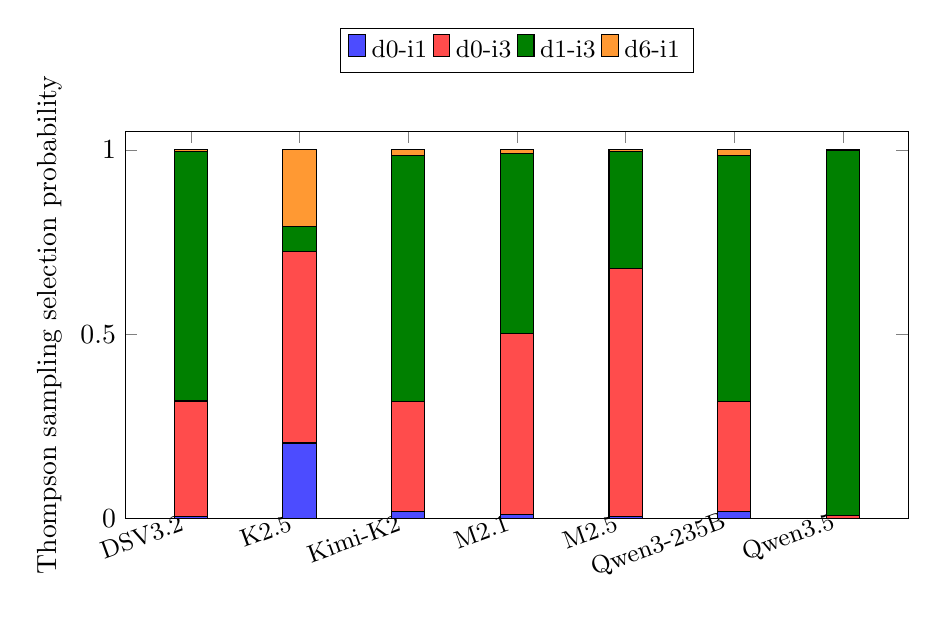
\begin{tikzpicture}
\begin{axis}[
  ybar stacked,
  bar width=12pt,
  width=0.95\linewidth,
  height=6.5cm,
  ymin=0, ymax=1.05,
  ylabel={Thompson sampling selection probability},
  symbolic x coords={DSV3.2,K2.5,Kimi-K2,M2.1,M2.5,Qwen3-235B,Qwen3.5},
  xtick=data,
  x tick label style={rotate=20,anchor=east,font=\small},
  legend style={at={(0.5,1.15)},anchor=south,legend columns=4,font=\small},
]
\addplot[fill=blue!70] coordinates {(DSV3.2,0.0047) (K2.5,0.2050) (Kimi-K2,0.0197) (M2.1,0.0103) (M2.5,0.0052) (Qwen3-235B,0.0197) (Qwen3.5,0.0006)};
\addplot[fill=red!70] coordinates {(DSV3.2,0.3142) (K2.5,0.5190) (Kimi-K2,0.2984) (M2.1,0.4906) (M2.5,0.6722) (Qwen3-235B,0.2984) (Qwen3.5,0.0077)};
\addplot[fill=green!50!black] coordinates {(DSV3.2,0.6757) (K2.5,0.0687) (Kimi-K2,0.6661) (M2.1,0.4897) (M2.5,0.3181) (Qwen3-235B,0.6661) (Qwen3.5,0.9912)};
\addplot[fill=orange!80] coordinates {(DSV3.2,0.0054) (K2.5,0.2073) (Kimi-K2,0.0158) (M2.1,0.0094) (M2.5,0.0045) (Qwen3-235B,0.0158) (Qwen3.5,0.0005)};
\legend{d0-i1,d0-i3,d1-i3,d6-i1}
\end{axis}
\end{tikzpicture}
\caption{Thompson sampling mode allocation per model (10{,}000 rounds). Each bar shows the probability that Thompson sampling would select each mode as optimal. Concentrated bars indicate high confidence; diffuse bars indicate mode-insensitivity.}
\label{fig:thompson-allocation}
\end{figure}

% === Latency Variability Table ===
\begin{table}[t]
\centering
\caption{Latency variability per model-mode (seconds). CV = coefficient of variation (std/mean).}
\label{tab:latency-variability}
\begin{tabular}{llrrrrrr}
\toprule
Model & Mode & $n$ & Mean & Std & CV & Min & Max \\
\midrule
  M2.1 & d0-i1 & 8 & 11.9 & 8.7 & 0.73 & 2.5 & 30.7 \\
  M2.1 & d1-i3 & 8 & 7.4 & 3.6 & 0.48 & 3.1 & 14.4 \\
  M2.1 & d6-i1 & 8 & 6.9 & 3.3 & 0.47 & 3.3 & 13.0 \\
  M2.1 & d0-i3 & 8 & 12.0 & 9.4 & 0.78 & 4.7 & 32.4 \\
  M2.5 & d0-i1 & 6 & 13.4 & 8.8 & 0.66 & 5.5 & 32.0 \\
  M2.5 & d1-i3 & 8 & 17.2 & 6.3 & 0.36 & 9.9 & 24.4 \\
  M2.5 & d6-i1 & 8 & 8.0 & 4.7 & 0.58 & 3.1 & 14.5 \\
  M2.5 & d0-i3 & 8 & 13.4 & 7.6 & 0.56 & 6.2 & 26.6 \\
  Qwen3-235B & d0-i1 & 8 & 25.5 & 21.8 & 0.86 & 8.3 & 77.3 \\
  Qwen3-235B & d1-i3 & 8 & 36.4 & 28.0 & 0.77 & 13.0 & 95.8 \\
  Qwen3-235B & d6-i1 & 8 & 30.0 & 28.5 & 0.95 & 8.4 & 98.0 \\
  Qwen3-235B & d0-i3 & 8 & 43.9 & 29.2 & 0.67 & 15.9 & 101.5 \\
  Qwen3.5 & d0-i1 & 8 & 11.4 & 6.5 & 0.57 & 4.3 & 23.5 \\
  Qwen3.5 & d1-i3 & 8 & 11.9 & 5.2 & 0.44 & 5.5 & 23.4 \\
  Qwen3.5 & d6-i1 & 8 & 12.9 & 10.2 & 0.79 & 4.9 & 36.4 \\
  Qwen3.5 & d0-i3 & 8 & 19.5 & 14.2 & 0.73 & 4.9 & 48.6 \\
  DSV3.2 & d0-i1 & 8 & 31.5 & 10.4 & 0.33 & 12.3 & 50.4 \\
  DSV3.2 & d1-i3 & 7 & 51.1 & 25.5 & 0.50 & 22.1 & 85.3 \\
  DSV3.2 & d6-i1 & 8 & 32.5 & 15.5 & 0.48 & 14.9 & 57.9 \\
  DSV3.2 & d0-i3 & 8 & 42.5 & 16.8 & 0.40 & 26.8 & 77.1 \\
  Kimi-K2 & d0-i1 & 8 & 12.0 & 5.5 & 0.46 & 5.4 & 20.2 \\
  Kimi-K2 & d1-i3 & 6 & 65.0 & 25.7 & 0.40 & 18.9 & 99.1 \\
  Kimi-K2 & d6-i1 & 7 & 23.0 & 22.7 & 0.98 & 7.1 & 72.5 \\
  Kimi-K2 & d0-i3 & 8 & 26.8 & 18.4 & 0.69 & 6.6 & 66.5 \\
  K2.5 & d0-i1 & 8 & 39.1 & 24.1 & 0.62 & 9.4 & 73.5 \\
  K2.5 & d1-i3 & 8 & 28.6 & 23.3 & 0.81 & 8.4 & 86.2 \\
  K2.5 & d6-i1 & 8 & 27.1 & 20.2 & 0.75 & 7.1 & 64.0 \\
  K2.5 & d0-i3 & 8 & 38.1 & 28.6 & 0.75 & 13.3 & 107.9 \\
\bottomrule
\end{tabular}
\end{table}

% === Latency CV Figure ===
\begin{figure}[t]
\centering
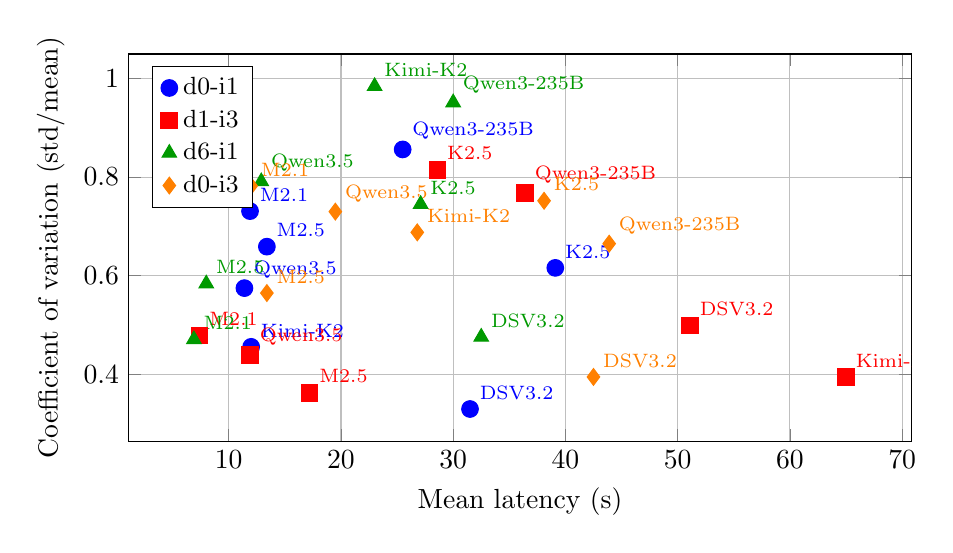
\begin{tikzpicture}
\begin{axis}[
  width=0.95\linewidth,
  height=6.5cm,
  xlabel={Mean latency (s)},
  ylabel={Coefficient of variation (std/mean)},
  grid=major,
  legend style={at={(0.03,0.97)},anchor=north west,font=\small},
]
\addplot[only marks,mark=*,mark size=3pt,blue] coordinates {(11.9,0.731) (13.4,0.659) (25.5,0.856) (11.4,0.575) (31.5,0.330) (12.0,0.456) (39.1,0.616)};
\node[anchor=south west,font=\scriptsize,blue] at (axis cs:11.9,0.731) {M2.1};
\node[anchor=south west,font=\scriptsize,blue] at (axis cs:13.4,0.659) {M2.5};
\node[anchor=south west,font=\scriptsize,blue] at (axis cs:25.5,0.856) {Qwen3-235B};
\node[anchor=south west,font=\scriptsize,blue] at (axis cs:11.4,0.575) {Qwen3.5};
\node[anchor=south west,font=\scriptsize,blue] at (axis cs:31.5,0.330) {DSV3.2};
\node[anchor=south west,font=\scriptsize,blue] at (axis cs:12.0,0.456) {Kimi-K2};
\node[anchor=south west,font=\scriptsize,blue] at (axis cs:39.1,0.616) {K2.5};
\addplot[only marks,mark=square*,mark size=3pt,red] coordinates {(7.4,0.479) (17.2,0.363) (36.4,0.768) (11.9,0.440) (51.1,0.499) (65.0,0.395) (28.6,0.815)};
\node[anchor=south west,font=\scriptsize,red] at (axis cs:7.4,0.479) {M2.1};
\node[anchor=south west,font=\scriptsize,red] at (axis cs:17.2,0.363) {M2.5};
\node[anchor=south west,font=\scriptsize,red] at (axis cs:36.4,0.768) {Qwen3-235B};
\node[anchor=south west,font=\scriptsize,red] at (axis cs:11.9,0.440) {Qwen3.5};
\node[anchor=south west,font=\scriptsize,red] at (axis cs:51.1,0.499) {DSV3.2};
\node[anchor=south west,font=\scriptsize,red] at (axis cs:65.0,0.395) {Kimi-K2};
\node[anchor=south west,font=\scriptsize,red] at (axis cs:28.6,0.815) {K2.5};
\addplot[only marks,mark=triangle*,mark size=3pt,green!60!black] coordinates {(6.9,0.471) (8.0,0.584) (30.0,0.951) (12.9,0.791) (32.5,0.476) (23.0,0.984) (27.1,0.745)};
\node[anchor=south west,font=\scriptsize,green!60!black] at (axis cs:6.9,0.471) {M2.1};
\node[anchor=south west,font=\scriptsize,green!60!black] at (axis cs:8.0,0.584) {M2.5};
\node[anchor=south west,font=\scriptsize,green!60!black] at (axis cs:30.0,0.951) {Qwen3-235B};
\node[anchor=south west,font=\scriptsize,green!60!black] at (axis cs:12.9,0.791) {Qwen3.5};
\node[anchor=south west,font=\scriptsize,green!60!black] at (axis cs:32.5,0.476) {DSV3.2};
\node[anchor=south west,font=\scriptsize,green!60!black] at (axis cs:23.0,0.984) {Kimi-K2};
\node[anchor=south west,font=\scriptsize,green!60!black] at (axis cs:27.1,0.745) {K2.5};
\addplot[only marks,mark=diamond*,mark size=3pt,orange] coordinates {(12.0,0.782) (13.4,0.565) (43.9,0.665) (19.5,0.730) (42.5,0.395) (26.8,0.688) (38.1,0.752)};
\node[anchor=south west,font=\scriptsize,orange] at (axis cs:12.0,0.782) {M2.1};
\node[anchor=south west,font=\scriptsize,orange] at (axis cs:13.4,0.565) {M2.5};
\node[anchor=south west,font=\scriptsize,orange] at (axis cs:43.9,0.665) {Qwen3-235B};
\node[anchor=south west,font=\scriptsize,orange] at (axis cs:19.5,0.730) {Qwen3.5};
\node[anchor=south west,font=\scriptsize,orange] at (axis cs:42.5,0.395) {DSV3.2};
\node[anchor=south west,font=\scriptsize,orange] at (axis cs:26.8,0.688) {Kimi-K2};
\node[anchor=south west,font=\scriptsize,orange] at (axis cs:38.1,0.752) {K2.5};
\legend{d0-i1,d1-i3,d6-i1,d0-i3}
\end{axis}
\end{tikzpicture}
\caption{Latency mean vs coefficient of variation by model and mode. High CV indicates unstable response times. Ideal configurations are in the lower-left quadrant.}
\label{fig:latency-cv}
\end{figure}